\documentclass{article}
\usepackage{babel}
\usepackage[a4paper, top = 20mm, bottom=20mm, right=20mm, left=20mm]{geometry}
\usepackage{graphicx}
\usepackage{amsmath}
\usepackage{wrapfig}
\usepackage{xcolor}
\usepackage[hidelinks]{hyperref}
\usepackage{listingsutf8}
\usepackage{tocloft}
\setlength{\parindent}{3mm}
\setlength{\parskip}{5mm}
\linespread{1.65}
\renewcommand{\figurename}{Fig.}

\title{Sistemas de Información y Telemedicina II\thanks{\href{https://www.upv.es/titulaciones/GIB/indexc.html}{Grado en Ingeniería Biomédica, Escuela Técnica Superior de Ingenieros Industriales, Valencia, España.}} \\\textbf{Machine Learning para Mesotelioma Maligno}}
\author{
\href{mailto:irgarga4@etsii.upv.es}{Irene Estela García García}
\and
\href{mailto:ilcarjuc@etsii.upv.es}{Ilán Francisco Carretero Juchnowicz}
\and
\href{mailto:igamher@etsid.upv.es}{Ignacio Maria Amat Hernández}
}
\date{\today}

\lstset{
	language=Python,
	inputencoding=utf8/latin1,
	frame=single,
	numbers=left,
	basicstyle=\linespread{1.1}\ttfamily,
	mathescape,
	numberstyle=\color{gray},
	stringstyle=\color[HTML]{933797},
	commentstyle=\color[HTML]{228B22}\sffamily,
	emph={[2]from,import,pass,return}, emphstyle={[2]\color[HTML]{DD52F0}},
	emph={[3]range}, emphstyle={[3]\color[HTML]{D17032}},
	emph={[4]for,in,def}, emphstyle={[4]\color{blue}},
	showstringspaces=false,
	breaklines=true,
	prebreak=\mbox{{\color{gray}\tiny$\searrow$}},
	captionpos=b,
}


\newcommand{\diagram}[2]{
\subsection{#2}
\begin{figure}[h]
\centering
\includegraphics[width = 0.9\linewidth]{#1}
\caption{#2.}
\end{figure}
}

\newcommand{\incpng}[2]{
\begin{figure}[h]
\centering
\includegraphics[trim=3cm 3cm 3cm 0cm, width = 0.77\linewidth]{#1}
\caption{#2}
\end{figure}
}

\begin{document}
\maketitle
\newpage
\tableofcontents
\listoffigures
\lstlistoflistings
\newpage

\section{Análisis exploratorio}
\subsection{Tipos de datos}

Comenzamos analizando la base de datos,  consta de las siguientes
variables:
\\
\begin{lstlisting}[
	label=lst:cod1,
	caption = {Variables de la base de datos.},
	]
RangeIndex: 324 entries, 0 to 323
Data columns (total 30 columns):
 #   Column                            Non-Null Count  Dtype
---  ------                            --------------  -----
 0   age                               324 non-null    float64
 1   gender                            324 non-null    int64
 2   city                              324 non-null    int64
 3   asbestos exposure                 324 non-null    int64
 4   duration of asbestos exposure     324 non-null    float64
 5   keep side                         324 non-null    int64
 6   duration of symptoms              324 non-null    float64
 7   dyspnoea                          324 non-null    int64
 8   ache on chest                     324 non-null    int64
 9   weakness                          324 non-null    int64
 10  habit of cigarette                324 non-null    int64
 11  performance status                324 non-null    int64
 12  white blood                       324 non-null    float64
 13  cell count (WBC)                  324 non-null    int64
 14  hemoglobin (HGB)                  324 non-null    int64
 15  platelet count (PLT)              324 non-null    float64
 16  sedimentation                     324 non-null    float64
 17  blood lactic dehydrogenise (LDH)  324 non-null    float64
 18  alkaline phosphatise (ALP)        324 non-null    float64
 19  total protein                     324 non-null    float64
 20  albumin                           324 non-null    float64
 21  glucose                           324 non-null    float64
 22  pleural lactic dehydrogenise      324 non-null    float64
 23  pleural protein                   324 non-null    float64
 24  pleural albumin                   324 non-null    float64
 25  pleural glucose                   324 non-null    float64
 26  pleural effusion                  324 non-null    float64
 27  pleural thickness on tomography   324 non-null    float64
 28  pleural level of acidity (pH)     324 non-null    float64
 29  C-reactive protein (CRP)          324 non-null    int64
dtypes: float64(18), int64(12)
memory usage: 76.1 KB
\end{lstlisting}

Nuestra base de datos consta de 324 entradas, cada una  con 30
variables. Todos los valores son \lstinline{floats} e
\lstinline{ints}, además no tenemos ningún \lstinline{NULL}.

\newpage
\diagram {../images/boxplot.pdf}{Caja bigotes}

Vemos que no hay diferencias notables entre los diagramas  de  nuestra
población   de	 pacientes   sanos   y	 enfermos.    Las   variables
\lstinline{PLT, PLT, glucosa} y \lstinline{PLD}  parecen  tener  datos
anómalos.

\newpage
\diagram {../images/histogram.pdf}{Histograma}

Como es de esperar tras juzgar los  diagramas  de  caja  bigotes,  los
histogramas también tienen una distribución casi idéntica. Lo único en
lo que se diferencian es  en  la  cuentas  totales,  ello  indica  que
tenemos  más  observaciones  de  pacientes  sanos  que	de   enfermos.

\newpage
\diagram {../images/kdens.pdf}{Kernel Density}

A diferencia de los histogramas, al  tratarse  con  densidades	no  se
observan diferencias por la  distinta  cantidad  de  observaciones  de
sanos y enfermos.  Únicamente vemos que las  distribuciones  son  casi
idénticas, como intuíamos de los histogramas.

\newpage
\diagram {../images/qqplot.pdf}{Cuantil - cuantil}

\newpage
\diagram {../images/corrtodas.pdf}{Correlaciones}

\newpage
\section{Extracción de Características}
\subsection{Filter methods}

\begin{lstlisting}[
	label=lst:cod2,
	caption = {Selecci\'on de variables seg\'un \lstinline{fscore}},
	]
Ranking    Variable
-------    --------
 1         pleural level of acidity (pH)
 2         C-reactive protein (CRP)
 3         gender
 4         pleural lactic dehydrogenise
 5         pleural effusion
 6         pleural glucose
 7         pleural albumin
 8         keep side
 9         blood lactic dehydrogenise (LDH)
10         total protein
11         alkaline phosphatise (ALP)
12         white blood
13         performance status
14         cell count (WBC)
15         habit of cigarette
16         pleural protein
17         duration of asbestos exposure
18         city
19         dyspnoea
20         ache on chest
21         sedimentation
22         asbestos exposure
23         platelet count (PLT)
24         glucose
25         albumin
26         duration of symptoms
27         weakness
28         age
29         hemoglobin (HGB)
30         pleural thickness on tomography
\end{lstlisting}

Usando la puntuación de \textit{Fisher} clasificamos las
características de mayor a menor relevancia a la hora de resolver el
problema de clasificación

\newpage
\subsection{Wrapper methods}
\begin{lstlisting}[
	label=lst:cod3,
	caption = {Mejores variables seg\'un \lstinline{SFS} y \lstinline{SBS}},
	]
0.6782828282828283
Sequential Forward  Selection ('asbestos exposure',
				'keep side',
				'weakness',
				'cell count (WBC)',
				'platelet count (PLT)',
				'alkaline phosphatise (ALP)',
				'glucose',
				'pleural protein',
				'pleural glucose',
				'C-reactive protein (CRP)')

0.5414285714285715
Sequential Backward Selection ('city',
			       'asbestos exposure',
			       'keep side',
			       'duration of symptoms',
			       'ache on chest',
			       'performance status',
			       'platelet count (PLT)',
			       'alkaline phosphatise (ALP)',
			       'pleural albumin',
			       'C-reactive protein (CRP)')
\end{lstlisting}

Una selección secuencial hacia adelante y hacia atrás con un modelo de
\lstinline{randomforest} con 100 estimadores y 10 parámetros
calculamos una precisión del 67\%. Los resultados son menores cuando
hacemos la selección hacia atrás. También lo hemos intentado con un
modelo \lstinline{knn}, los resultados son peores en torno al 50\%.

\newpage
\subsection{PCA}

\begin{figure}[h]
\centering
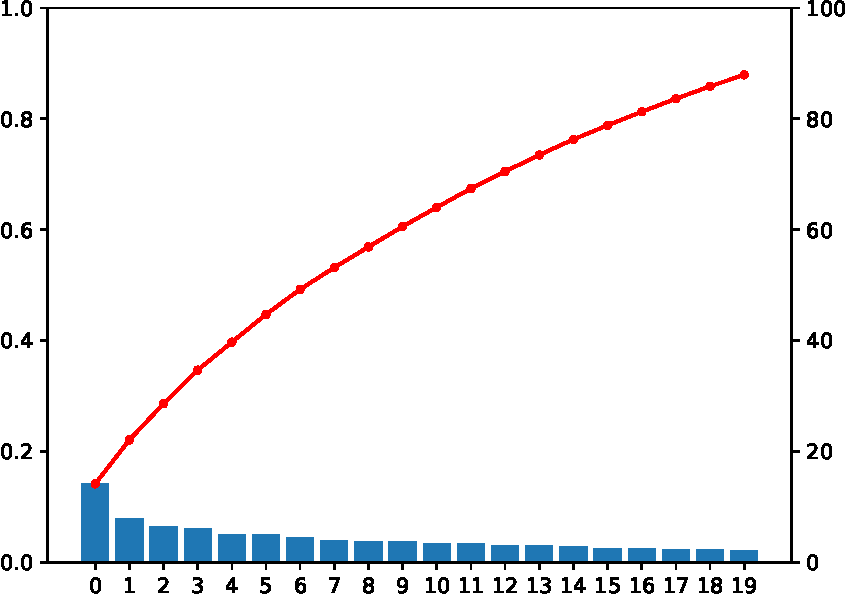
\includegraphics[width = 0.9\linewidth]{../images/pareto.pdf}
\caption{Diagrama de pareto.}
\end{figure}

Calculando el diagrama de pareto vemos que necesitaríamos entorno a 17
componentes para explicar el 80\% de la varianza de los datos. Con
estos resultados vemos que  será difícil reducir al dimensionalidad
en componentes principales.

\newpage
\section{Modelos de Clasificación}

\begin{lstlisting}[
	label=lst:cod3,
	caption = {Modelos de clasificaci\'on en Python},
	]
from sklearn.discriminant_analysis import LinearDiscriminantAnalysis

modeloLDA = LinearDiscriminantAnalysis ();

from sklearn.discriminant_analysis import QuadraticDiscriminantAnalysis

modeloQDA = QuadraticDiscriminantAnalysis ();

from sklearn.neighbors import KNeighborsClassifier

modeloKNN   = KNeighborsClassifier (n_neighbors = 50)

from sklearn.ensemble import RandomForestClassifier

modelFOREST = RandomForestClassifier (
        n_estimators = 100,
        criterion = 'gini',
        )

from neupy import algorithms

modeloPNN = algorithms.PNN (
        std=5,
        verbose=False,
        )

from sklearn.neural_network import MLPClassifier as MLP

modeloMLP = MLP(
        hidden_layer_sizes = (175, 100, 50, 25, ),
        max_iter = 500,
        random_state = 1)

from sklearn import svm

modeloSVM = svm.LinearSVC()
\end{lstlisting}

\begin{table}[h!]
\centering
\begin{tabular}{|c|c|c|c|c|c|c|c|c|}
\hline
Model  & TP    & FP    & FN    & TN   & Accuracy & Sensitivity & Specificity & Time\\
\hline
   LDA & 58.45 & 10.60 & 21.31 & 7.63 &  0.67    & 0.73        & 0.42        & 5.21\\
   QDA & 55.93 & 12.94 & 22.43 & 6.70 &  0.64    & 0.71        & 0.34        & 4.58\\
   KNN & 68.99 & 0.00  & 29.01 & 0.00 &  0.70    & 0.70        & nan         & 9.74\\
FOREST & 66.55 & 2.54  & 23.96 & 4.95 &  0.73    & 0.74        & 0.66        & 181.79\\
   SVM & 45.93 & 22.88 & 19.88 & 9.31 &  0.56    & 0.70        & 0.29        & 20.90\\
   PNN & 61.88 & 7.06  & 25.27 & 3.78 &  0.67    & 0.71        & 0.35        & 9.15\\
   MLP & 48.57 & 20.53 & 20.42 & 8.48 &  0.58    & 0.70        & 0.29        & 287.44\\
\hline
\end{tabular}
\caption{Resultados agregados tras 1000 repeticiones.}
\label{table:}
\end{table}

\section{Interfaz}

\incpng{../images/s1.png} {Ventana principal.}

Ventana principal de nuestra interfaz. A la izquierda campos de texto
para introducir las variables, se muestra entre paréntesis el rango de
dicha variable en nuestra base de datos.

\begin{figure}[h]
\centering
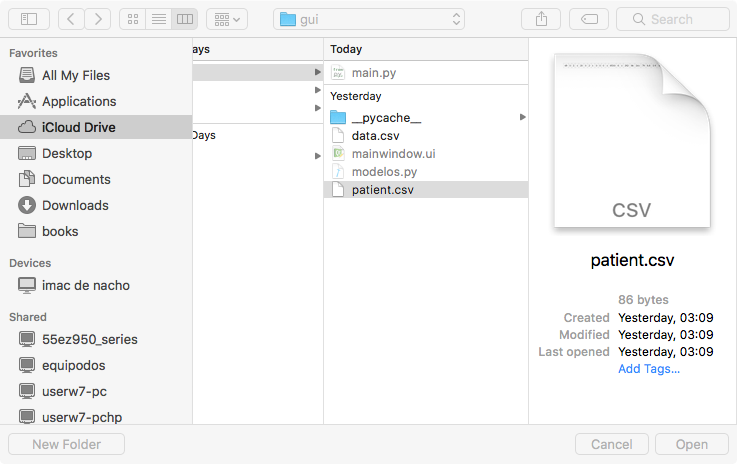
\includegraphics[trim=3cm 1cm 3cm 0cm, width = 0.5\linewidth]{../images/s2.png}
\caption{Selección de paciente.}
\end{figure}

Para hacer mas cómodo su uso y evitar tener que introducir 30+
variables a mano, al presionar Ctrl + O se abre una ventana para
seleccionar un archivo .csv, contiene todos los valores para un
paciente separados por comas.

\newpage
\incpng{../images/s3.png} {Importación paciente.}

Al importar el paciente se rellenan automáticamente las variables, se
pueden comprobar y editar si fuera necesario.

\incpng{../images/s4.png} {Cargar variables.}

Al presionar Enter con el teclado o el botón 'Leer Vars' con  el
ratón se guardan las variables en la memoria del programa. Para
actualizar una variable no hay más que introducir un nuevo valor y pulsar
enter o el ratón.
Para cargar el modelo se presiona Ctrl + M, o se elige desde el menú.
Aparece una venta para seleccionar el archivo .py con los modelos en
python.

\newpage
\begin{figure}[h]
\centering
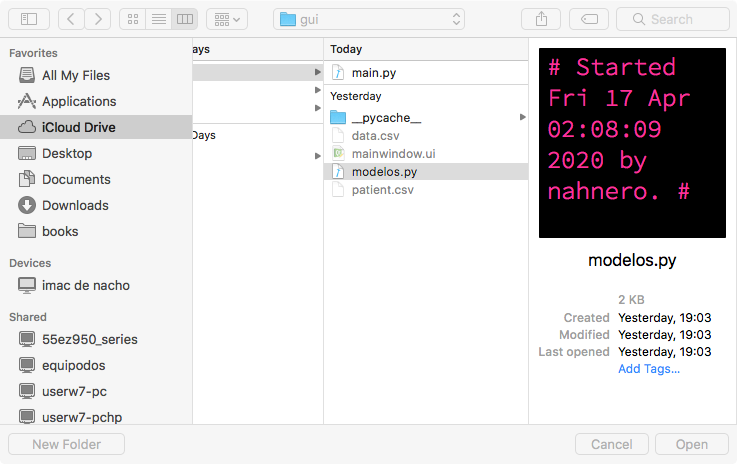
\includegraphics[trim=3cm 1cm 3cm 0cm, width = 0.5\linewidth]{../images/s5.png}
\caption{Selección de modelos.}
\end{figure}

Una vez cargados los modelos se selecciona que modelo se desea
ejecutar, los botones son mutuamente excluyentes. Al ejecutarse el
modelo se generan las métricas de evaluación a la derecha y el
diagnóstico.

\incpng{../images/s6.png} {Selección de modelos.}

Cuando se selecciona otro modelo se revalúa al paciente, cada modelo
tiene unas características diferentes en cuanto a exactitud,
sensitividad y especificidad. En función de lo que se busque se puede
seleccionar un modelo adecuado.

\newpage
\subsection{Interfaz sin  opciones}

Esta versión restringe al usuario a usar un modelo predeterminado.
Al pulsar el botón ejecutar, después de haber introducido los datos del
paciente se calcula el modelo y se presentan los resultados.

\incpng{../images/s8.png} {Versión limitada para médicos.}













\end{document}
